\documentclass[11pt]{article}
\usepackage{enumitem}
\usepackage{listings}
\usepackage{tikz}
\usepackage{url}
%\usepackage{algorithm2e}
\usetikzlibrary{arrows,automata,shapes}
\tikzstyle{block} = [rectangle, draw, fill=blue!20, 
    text width=5em, text centered, rounded corners, minimum height=2em]
\tikzstyle{bt} = [rectangle, draw, fill=blue!20, 
    text width=4em, text centered, rounded corners, minimum height=2em]

\lstset{ %
language=Java,
basicstyle=\ttfamily,commentstyle=\scriptsize\itshape,showstringspaces=false,breaklines=true,numbers=left}

\newtheorem{defn}{Definition}
\newtheorem{crit}{Criterion}

\newcommand{\handout}[5]{
  \noindent
  \begin{center}
  \framebox{
    \vbox{
      \hbox to 5.78in { {\bf Software Testing, Quality Assurance and Maintenance } \hfill #2 }
      \vspace{4mm}
      \hbox to 5.78in { {\Large \hfill #5  \hfill} }
      \vspace{2mm}
      \hbox to 5.78in { {\em #3 \hfill #4} }
    }
  }
  \end{center}
  \vspace*{4mm}
}

\newcommand{\lecture}[4]{\handout{#1}{#2}{#3}{#4}{Lecture #1}}
\topmargin 0pt
\advance \topmargin by -\headheight
\advance \topmargin by -\headsep
\textheight 8.9in
\oddsidemargin 0pt
\evensidemargin \oddsidemargin
\marginparwidth 0.5in
\textwidth 6.5in

\parindent 0in
\parskip 1.5ex
%\renewcommand{\baselinestretch}{1.25}

\usepackage{fontspec}
\setmonofont{Cousine}[Scale=MatchLowercase]

\begin{document}

\lecture{7 --- January 18, 2017}{Winter 2017}{Patrick Lam}{version 1}

\paragraph{Basic Blocks.} We can simplify a CFG by grouping together
statements which always execute together (in sequential programs):

\begin{center}
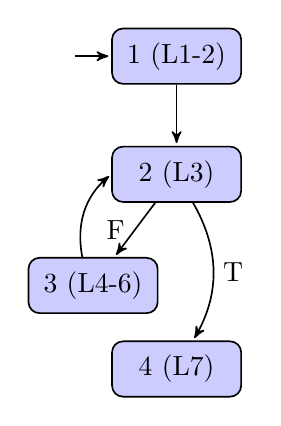
\begin{tikzpicture}[->,>=stealth',shorten >=1pt,auto,node distance=1.5cm,
                    semithick,initial text=]

  \node[initial,bt]   (1)                     {1 (L1-2)};
  \node[bt]           (2) [below of=1] {2 (L3)};
  \node[bt]           (3) [below left of=2,yshift=-1em] {3 (L4-6)};
  \node[bt]           (4) [below right of=3] {4 (L7)};

  \path (1) edge node {} (2)
        (2) edge node[left] {F} (3)
            edge [bend left] node {T} (4)
        (3) edge [bend left] node {} (2.west);
\end{tikzpicture}
\end{center}

We use the following definition:
\begin{defn}
A basic block is a sequence of instructions in the control-flow graph
that has one entry point and one exit point.
\end{defn}
We are usually interested in forming maximal basic blocks.
Note that a basic block may have multiple successors. However, there 
may not be any jumps into the middle of a basic block (which is
why statement {\tt l0} has its own basic block.)

\subsection*{Some Examples} We'll now see how to construct
control-flow graph fragments for various program constructs.

{\bf if statements:} One can put the conditions
(and hence uses) on the control-flow edges, rather than in the 
{\tt if} node. I prefer putting the condition in the node.

\begin{tabular}{ll|ll}
\begin{minipage}{.15\textwidth}
\scriptsize \begin{lstlisting}
if (z < 17)
  print (x);
else
  print (y);
\end{lstlisting}
\end{minipage} &
\begin{minipage}{.3\textwidth}
\begin{center}
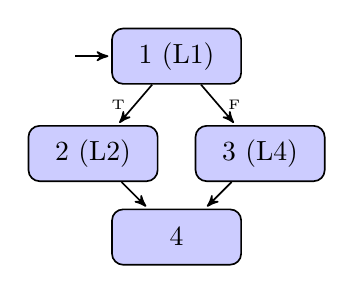
\begin{tikzpicture}[->,>=stealth',shorten >=1pt,auto,node distance=1.5cm,
                    semithick,initial text=]

  \node[initial,bt]   (1)                     {1 (L1)};
  \node[bt]           (2) [below left of=1,yshift=-0.5em] {2 (L2)};
  \node[bt]           (3) [below right of=1,yshift=-0.5em] {3 (L4)};
  \node[bt]           (4) [below left of=3] {4};

  \path (1) edge node[left] {\tiny T} (2)
        (1) edge node[right] {\tiny F} (3)
        (2) edge node {} (4)
        (3) edge node {} (4);
\end{tikzpicture}
\end{center}
\end{minipage}&
\begin{minipage}{.25\textwidth}
\begin{center}
\begin{tikzpicture}[->,>=stealth',shorten >=1pt,auto,node distance=1.5cm,
                    semithick,initial text=]

  \node[initial,bt]   (1)                     {1 (L1)};
  \node[bt]           (2) [below left of=1,yshift=-0.5em] {2 (L2)};
  \node[bt]           (4) [below left of=3] {3};

  \path (1) edge node[left] {\tiny T} (2)
        (1) edge node[right] {\tiny F} (4)
        (2) edge node {} (4);
\end{tikzpicture}
\end{center}
\end{minipage}
& \scriptsize \begin{minipage}{.2\textwidth}
\begin{lstlisting}
if (z < 17)
  print(x);
\end{lstlisting}
\end{minipage}
\end{tabular}

Short-circuit {\tt if} evaluation is more complicated; I recommend working it out yourself.
\newpage

{\bf case / switch statements:} 

\begin{tabular}{ll}
\begin{minipage}{.45\textwidth}
\begin{lstlisting}
switch (n) {
  case `I': ...; break;
  case `J': ...; // fall thru
  case `K': ...; break;
}
// ...
\end{lstlisting}
\end{minipage} &
\begin{minipage}{.4\textwidth}
\begin{center}
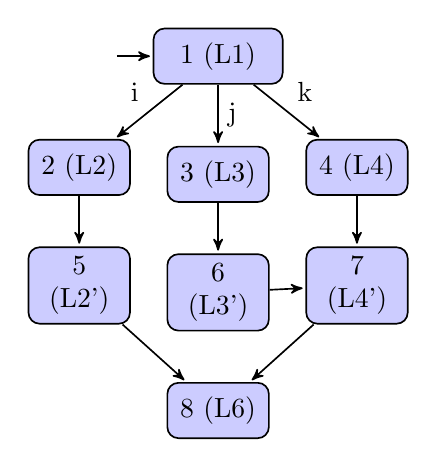
\begin{tikzpicture}[->,>=stealth',shorten >=1pt,auto,node distance=1.5cm,
                    semithick,initial text=]

  \node[initial,bt]   (1)                     {1 (L1)};
  \node[bt, text width=3em]           (2) [below left of=1,xshift=-2em,yshift=-1em]  {2 (L2)};
  \node[bt, text width=3em]           (3) [below of=1]   {3 (L3)};
  \node[bt, text width=3em]           (4) [below right of=1,xshift=2em,yshift=-1em]   {4 (L4)};
  \node[bt, text width=3em]           (5) [below of=2]  {5 (L2')};
  \node[bt, text width=3em]           (6) [below of=3]  {6 (L3')};
  \node[bt, text width=3em]           (7) [below of=4]  {7 (L4')};
  \node[bt, text width=3em]           (8) [below of=6]  {8 (L6)};

  \path 
  (1) edge node[left,yshift=0.7em] {i} (2)
  (1) edge node {j} (3)
  (1) edge node {k} (4)
  (2) edge node {} (5)
  (3) edge node {} (6)
  (4) edge node {} (7)
  (6) edge node {} (7)
  (5) edge node {} (8)
  (7) edge node {} (8);
\end{tikzpicture}
\end{center}
\end{minipage}
\end{tabular}

{\bf while statements:}

\begin{tabular}{ll}
\begin{minipage}{.2\textwidth}
\begin{lstlisting}
x = 0; y = 20;
while (x < y) {
  x ++; y --;
}
\end{lstlisting}
\end{minipage} &
\begin{minipage}{.4\textwidth}
\begin{center}
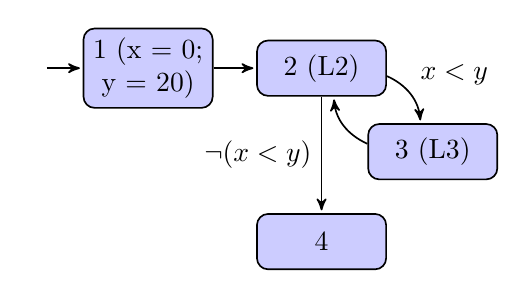
\begin{tikzpicture}[->,>=stealth',shorten >=1pt,auto,node distance=1.5cm,
                    semithick,initial text=]

  \node[initial,bt]   (1)                     {1 (x = 0; y = 20)};
  \node[bt]           (2) [right of=1,xshift=2em]        {2 (L2)};
  \node[bt]           (3) [below right of=2,xshift=1em]  {3 (L3)};
  \node[bt]           (4) [below of=2,yshift=-2em]   {4};

  \path (1) edge node {} (2)
  (2) edge [bend left] node {$x < y$} (3)
  (3) edge [bend left] node {} (2)
  (2) edge node[left] {$\neg (x < y)$} (4);
\end{tikzpicture}
\end{center}
\end{minipage}
\end{tabular}

Note that arbitrarily complicated structures may occur inside
the loop body.

    {\bf for statements:} 

\begin{tabular}{ll}
\begin{minipage}{.5\textwidth}
\begin{lstlisting}
for (int i = 0; i < 57; i++) {
  if (i % 3 == 0) {
    print (i);
  }
}
\end{lstlisting}
\end{minipage} & \begin{minipage}{.4\textwidth}
  (an exercise for the reader; \\ 
we saw one earlier!)
\end{minipage}
\end{tabular}

This example uses Java's enhanced for loops, which iterates over all of the elements
in the {\tt widgetList}:

\begin{lstlisting}[basicstyle=\scriptsize \ttfamily]
for (Widget w : widgetList) {
  decorate(w);
}
\end{lstlisting}

I will accept the simplified CFG or the more useful one on the right:

\begin{tabular}{ll}
\begin{minipage}{.4\textwidth}
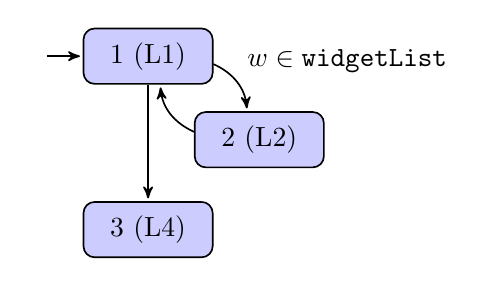
\begin{tikzpicture}[->,>=stealth',shorten >=1pt,auto,node distance=1.5cm,
                    semithick,initial text=]

  \node[initial,bt]   (1)                     {1 (L1)};
  \node[bt]           (3) [below right of=1,xshift=1em]  {2 (L2)};
  \node[bt]           (4) [below of=1,yshift=-2em]   {3 (L4)};

  \path 
  (1) edge [bend left] node {$w \in \mbox{\tt widgetList}$} (3)
  (3) edge [bend left] node {} (1)
  (1) edge node[left] {} (4);
\end{tikzpicture}
\end{minipage} &
\begin{minipage}{.5\textwidth}
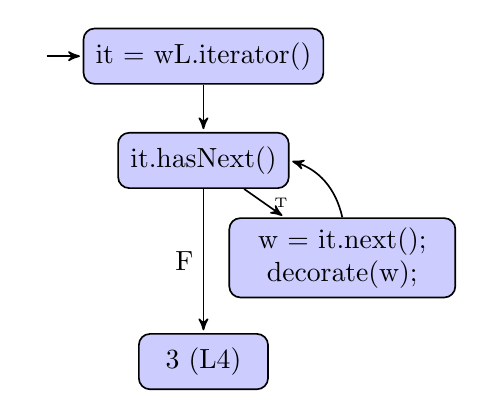
\begin{tikzpicture}[->,>=stealth',shorten >=1pt,auto,node distance=1.5cm,
                    semithick,initial text=]

  \node[initial,bt,text width=8em]   (1)                     {it = wL.iterator()};
  \node[bt,text width=5.5em]            (2) [below of=1,yshift=.5em] {it.hasNext()};
  \node[bt,text width=7.5em]           (3) [below right of=2,xshift=2em,yshift=-.5em]  {w = it.next(); decorate(w);};
  \node[bt]           (4) [below of=2,yshift=-3em]   {3 (L4)};

  \path (1) edge node {} (2)
        (2) edge node[right] {\tiny T} (3)
        (3.north) edge [bend right] node {} (2.east)
        (2) edge node[left] {F} (4);
%  (1) edge [bend left] node {$w \in \mbox{\tt widgetList}$} (3)
%  (3) edge [bend left] node {} (1)
%  (1) edge node[left] {} (4);
\end{tikzpicture}
\end{minipage}
\end{tabular}


\end{document}
